\documentclass{article}
\usepackage{tikz,tcolorbox}
\usepackage{array} % For customizing tables
\usepackage{booktabs} % For better horizontal lines
\usepackage[a4paper, paperwidth=25cm, paperheight=25.5cm, left=2cm, right=2cm, top=2cm, bottom=2cm]{geometry}
\usepackage{multicol}
\usepackage{amsmath}
\usepackage{pgfplots}
\usetikzlibrary{patterns}
\definecolor{greenPlot}{HTML}{14C877}
\definecolor{orangePlot}{HTML}{EA6E12}
\definecolor{purplePlot}{HTML}{4C12EA}
\definecolor{blueArea}{HTML}{10D9EE}
\begin{document}
\renewcommand{\arrayrulewidth}{0.75mm} % Set line thickness
\setlength{\tabcolsep}{12pt} % Set horizontal padding
\renewcommand{\arraystretch}{1.5} % Set vertical padding (1.0 is default)
\section{Opration Research}
\subsection{What's Operations Research?}
\begin{prettyBox}{Definition}{box}
Operations Research (\textbf{OR}) is an interdisciplinary field that uses mathematical models, statistical analysis, 
and optimization techniques to help solve complex decision-making problems and achieve the most efficient outcomes.
\noindent it involves the use of several key techniques, including:

\begin{itemize}
    \item \textbf{\underline{Optimization}}: Finding the best solution based on given criteria.
    \item \textbf{\underline{Mathematical Modeling}}: Representing real-world scenarios through mathematical equations and models.
    \item \textbf{\underline{Statistical Analysis}}: Using data to analyze and predict outcomes.
    \item \textbf{\underline{Simulation}}: Testing strategies in a controlled model environment.
\end{itemize}
The goal of Operations Research is to offer data-driven insights and methods that lead to more informed, optimized decisions.
\end{prettyBox}

\subsection{Origin of Operations Research}

\begin{prettyBox}{Origin}{box}
Operations Research (\textbf{OR}) originated during World War II, when the British government assembled a team of analysts, 
scientists, engineers, and military officers to study complex operational problems such as : air defense, bombing strategies, 
convoy routing, and other crucial military operations . Using mathematical models and data analysis, the team simulated various scenarios 
to predict outcomes and recommend optimal decisions. The success of these methods in improving military strategy inspired 
other nations to adopt similar approaches.This eventually led to the formalization of OR as a scientific discipline after the war.
\end{prettyBox}

\subsection{Types of Problems Treated by OR}

\begin{prettyBox}{Types Of Problems}{box}
Operations Research (\textbf{OR}) focuses on solving real-world problems by finding the most optimal decisions.The types of problems OR addresses can generally be categorized as:

\begin{itemize}
    \item \textbf{\underline{Maximization}}: Achieving the highest possible value for an objective, such as maximizing profits, productivity, or efficiency. 
        \begin{itemize}
            \item Example: Maximizing a company's revenue by determining the most profitable product mix.
        \end{itemize}
    
    \item \textbf{\underline{Minimization}}: Reducing or minimizing undesirable factors, such as costs, time, or resource consumption.
        \begin{itemize}
            \item Example: Minimizing the cost of materials in manufacturing while maintaining quality standards.
        \end{itemize}

    \item \textbf{\underline{Optimization}}: Finding the best possible solution from multiple alternatives, often involving both maximization and minimization aspects. 
        \begin{itemize}
            \item Example: Finding the shortest path in a transportation network or optimizing team roles in a project.
        \end{itemize}
\end{itemize}
\end{prettyBox}

\subsection{Algorithm Complexity}

\begin{prettyBox}{Algorithm Complexity}{box}
Algorithm complexity refers to the amount of computational resources an algorithm uses. These resources are typically categorized as:

\begin{itemize}
    \item \textbf{Time Complexity}: The amount of time it takes for an algorithm to run, depending on the size of the input.
    It is commonly expressed using Big O notation (e.g., \(O(n)\), \(O(\log n)\)), which describes the algorithm's growth rate
    as the input size increases.
    
    \item \textbf{Space Complexity}: The amount of memory or space an algorithm requires. This is influenced by the number and 
    size of variables, data structures, and other memory-using elements.
\end{itemize}

Minimizing both time and space complexity is crucial when developing efficient algorithms, as it leads to more optimal performance, especially for large-scale problems.
\end{prettyBox}


\section{Linear Programming}
\subsection{What's Linear Programming ?}
\begin{tcolorbox}[title = Definition] 
Linear programming is a sub-branch of optimization techniques. It involves modeling real-life problems as
linear equations and inequalities and using specialized methods to find optimal solution(s), if they exist.
\end{tcolorbox}
\vspace{1cm}
\begin{center}
    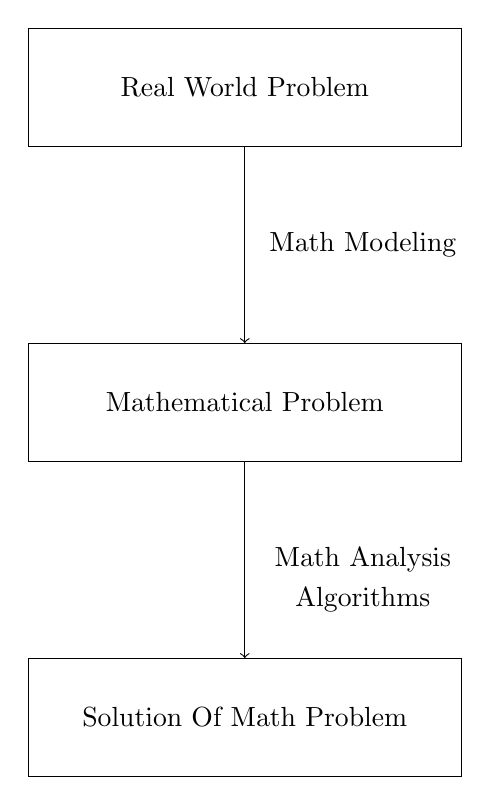
\begin{tikzpicture}
       \draw (0,0) rectangle (5.5,1.5);
       \node at (2.75,0.75) {Real World Problem};
      
       \draw[->] (2.75,0) -- (2.75,-2.5);
       \node at (4.25,-1.25) {Math Modeling};

       \draw (0,-4) rectangle (5.5,-2.5);
       \node at (2.75,-3.25) {Mathematical Problem};
      
       \draw[->] (2.75,-4) -- (2.75,-6.5);
       \node at (4.25,-5.25) {Math Analysis};
       \node at (4.25,-5.75) {Algorithms};
       
       \draw (0,-8) rectangle (5.5,-6.5);
       \node at (2.75,-7.25) {Solution Of Math Problem};
   \end{tikzpicture}
\end{center}
\vspace{1cm}
\subsection{Modeling}
\textbf{\large{\underline{Example :} Diet Problem}}\\

\vspace{0.25cm}
The Goal is to minimize food cost but to meet the minimum daily nutrition requirement
\vspace{1cm}
\begin{center}
\begin{tabular}{|c|c|c|c|c|c|}
    \hline
    Food & Units & Protein & Vit c & Iron & Price\\
    \hline
    Apples & 1 med & 0.4 & 6 & 0.4 & 8\\
    \hline
    Banana & 1 med & 1.2 & 10 & 0.6 & 10\\
    \hline
\end{tabular}
\end{center}

\vspace{1cm}

\begin{multicols}{2}
\textbf{\underline{Variables Definition:}}\\

Let \(x_1\) be the number of Daily Unit Appels.\\

Let \(x_2\) be the number of Daily Unit Banana.\\
\columnbreak

\textbf{\underline{Constraint:}} 

\[
\left\{
    \begin{array}{l}
        \forall x_1 , x_2 \geq 0 \quad \text{(Non-negative number of food item) ...C1}\\
        0.4x_1 + 1.2x_2  \geq 70 \quad \text{(Minimum Protein Daily) ...\textcolor{greenPlot}{C2}}\\ 
        6x_1 + 10x_2  \geq 50 \quad \text{(Minimum Vitamine c Daily) ...\textcolor{purplePlot}{C3}}\\
        0.4x_1 + 0.6x_2  \geq 12 \quad \text{(Minimum Iron Daily) ...\textcolor{orangePlot}{C4}}
   \end{array}
   \right.
\] 
\end{multicols}
\vspace{0.5cm}
\begin{tcolorbox}[title = Objectif Function]
\[
f(x_i) = Z = 8x_1 + 10x_2  
\]
\begin{center}
The goal is to minimize food cost by minmizing \(f(x_i)\), while meeting the minimum daily nutrition .
\end{center}
\end{tcolorbox}
\vspace{1cm} 
\textbf{\underline{Problem :}} Find the minimum of \(f(x_i)\) subject to the contraints\\

\subsection{Graph Model}
This model is used when the objective function has two variables. It consists of converting all inequalities
into equalities, drawing them as lines, and then identifying the feasible area where all conditions are met.
We then sweep the objective function \(Z\) across the plot until we find the optimal solution(s).

\begin{tcolorbox}[title=Note]
 \textbf{\underline{Solutions : }}
When solving a linear program, the solution can be:
\begin{itemize}
    \item \textbf{One or Multiple Optimal Solutions}: The feasible area is a polygon, and the points are solutions.
    \item \textbf{Infinitely Many Solutions}: If the feasible area is unbounded and the direction of increase or decrease 
for the objective function is towards \(\pm \infty\), then it will increase or decrease infinitely as we sweep the line.
    \item \textbf{No Solution}: If the feasible area does not exist (meaning \(\emptyset\)), it indicates that the
system has contradictions.
\end{itemize}


\textbf{\underline{Direction of Increase/Decrease:}}

\begin{itemize}
    \item \textbf{Both Positive} \((a > 0\) , \(b > 0)\): Since both coefficients are positive, \( Z \) increases as
\( x_1 \) and \( x_2 \) increase, and decreases as they decrease. The direction of increase is towards the right,
and the direction of decrease is towards the left.

    \item \textbf{Both Negative} \((a < 0\) , \(b < 0)\): The opposite of the positive case. Here, \( Z \) increases
as \( x_1 \) and \( x_2 \) decrease, and decreases as they increase. The direction of increase is towards the left,
while the direction of decrease is towards the right.

    \item \textbf{Different Signs} \((a\) and \(b\) have opposite signs): The direction is determined by 
the coefficient with the larger absolute value, \(\max(|a|, |b|)\). If this coefficient is positive, the direction 
of increase follows the same pattern as when both coefficients are positive. If this coefficient is negative, 
the direction of increase follows the pattern for both negative coefficients.
\end{itemize}
\end{tcolorbox}

\vspace{1cm}
\begin{center}
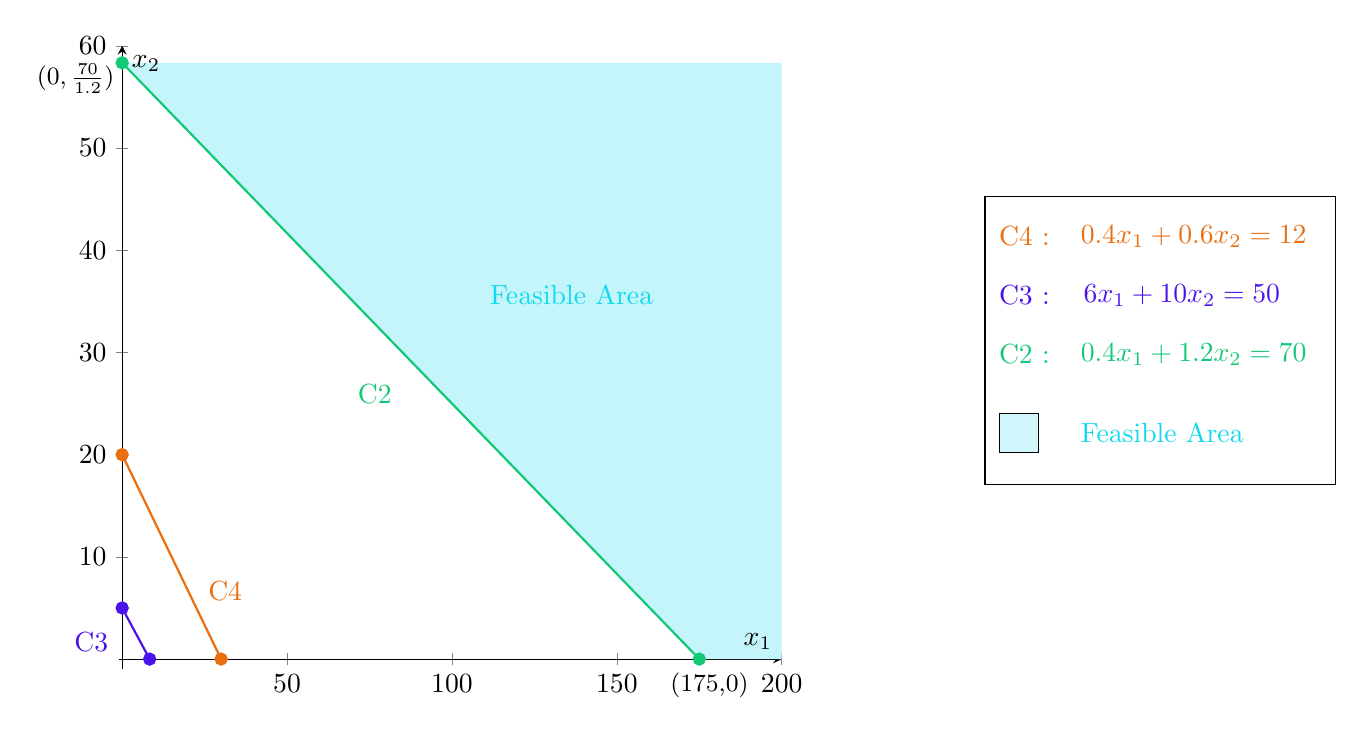
\begin{tikzpicture}
    \begin{axis}[
        height = 9.5cm,
        width = 10cm,
        axis lines = middle,           % Ensures axes cross at (0, 0)
        xlabel=$x_1$, 
        ylabel=$x_2$, 
        xmin = -1, xmax = 200,           % Set x-axis range
        ymin = -1, ymax = 60,           % Set y-axis range
       ytick={0,10,...,70},             % Y-tick values
        xtick={0,50,...,200},
    ]
  \addplot [draw=none, fill=blueArea!25] coordinates {(175,0) (200,0) (200,70/1.2) (0,70/1.2)}; 
  \addplot[thick, mark=*,color = greenPlot] coordinates {(175,0) (0,70/1.2)};
  %\addplot[color=red]coordinates{(150,8.5) (141,5)};
  \addplot[thick, mark=*, color = purplePlot] coordinates {(50/6,0) (0,5)};
  \addplot[thick, mark=*, color = orangePlot] coordinates {(30,0) (0,20)};
\end{axis}
\node at (7.5,-0.2){\small (175,0)};
\node at (-0.55,7.5){\small \((0,\frac{70}{1.2})\)};

\node at (1.35,1){\textcolor{orangePlot}{C4}};
\node at (-0.35,0.35){\textcolor{purplePlot}{C3}};
\node at (3.25,3.5){\textcolor{greenPlot}{C2}};
\node at (5.75,4.75){\textcolor{blueArea}{Feasible Area}};

\draw (11,2.35) rectangle (15.45,6);
\node at (11.5,5.5){\textcolor{orangePlot}{C4 :}};
\node at (13.65,5.5){\textcolor{orangePlot}{\(0.4x_1 + 0.6x_2  = 12 \)}};
\node at (11.5,4.75){\textcolor{purplePlot}{C3 :}};
\node at (13.5,4.75){\textcolor{purplePlot}{\(6x_1 + 10x_2 = 50\)}};
\node at (11.5,4){\textcolor{greenPlot}{C2 :}};
\node at (13.65,4){\textcolor{greenPlot}{\(0.4x_1 + 1.2x_2 = 70\)}};

\draw[fill=blueArea!20] (11.18,2.75) rectangle (11.68,3.25);
\node at (13.25,3){\textcolor{blueArea}{Feasible Area}};

\end{tikzpicture}
\end{center}

\subsubsection*{\underline{Solution}}

The blue area in the plot represents the feasible region, so the optimal solution(s) must be within this area. Since
the objective function \( Z \) increases towards the right (due to both coefficients being positive) and we want to
minimize \( Z \), we need to sweep the objective function line towards the leftmost boundary of the polygon. Thus,
the optimal solution is located at the leftmost point of the polygon, which is at \((0, \frac{70}{1.2})\). Therefore,
the optimal solution is \((0, \frac{70}{1.2})\) with \( Z = 8 \times 0 + 10 \times \frac{70}{1.2} = 583.33 \).


\end{document}
